\documentclass[../../../main.tex]{subfiles}

\begin{document}

\section{Geometry}

Unlike other fields in math olympiad, I think geometry is the section
that really need strong foundations with fundamental topics.
Assuming that we are aware of basic topics like similar triangles,
angle relationship between a tangent line and the inscribed triangle,
the relationship between arc length and angle in a circle, and more
foundational topics related to circles and points in triangles,
let's discuss some of the theorems that are necessary to understand
future topics.

Also please note that this section is quite terse with less
explanations and proofs. The latter section will prove the theorems
because we need to memorize the proofs to actually use them in the
exam, but the theorems mentioned here are considered common knowledge
and generally not required to prove them. But please don't quote me on
this because it depends on the exams and countries. Also because I
assume we are already familiar with the many of the topics here,
let's quickly go through them!

\begin{theorem}{Menelaus' Theorem}{Menelaus' Theorem}
Given a triangle $ABC$, let the transversal line $XY$ cut the triangle
and intersect $AC$ at $Z$. The, the following equation holds.
\[
\frac{BY}{YC} \cdot \frac{CZ}{ZA} \cdot \frac{AX}{XB} = 1
\]
\end{theorem}

Here is a diagram that manifests the theorem.

\begin{figure}[H]
\centering
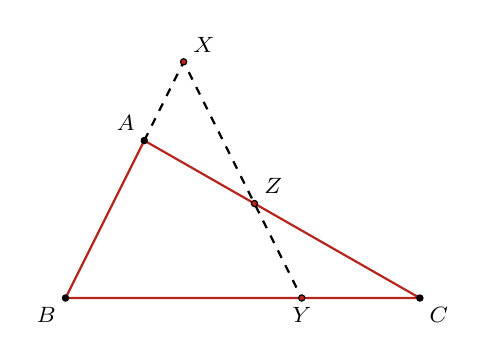
\begin{tikzpicture}[scale=0.5]
    \coordinate (A) at (2,4);
    \coordinate (B) at (0,0);
    \coordinate (C) at (9,0);
    \coordinate (X) at (3,6);
    \coordinate (Y) at (6,0);
    \coordinate (Z) at (4.8,2.4);

    \draw[thick, BrickRed] (A) -- (B) -- (C) -- cycle;
    \draw[thick, dashed] (A) -- (X) -- (Y);

    \draw[fill=black] (A) circle (0.08)
        node[above left] {\footnotesize $A$};
    \draw[fill=black] (B) circle (0.08)
        node[below left] {\footnotesize $B$};
    \draw[fill=black] (C) circle (0.08)
        node[below right] {\footnotesize $C$};
    \draw[fill=BrickRed] (X) circle (0.08)
        node[above right] {\footnotesize $X$};
    \draw[fill=BrickRed] (Y) circle (0.08)
        node[below] {\footnotesize $Y$};
    \draw[fill=BrickRed] (Z) circle (0.08)
        node[above right] {\footnotesize $Z$};
\end{tikzpicture}
\end{figure}

The equation can be quite hard to memorize as is, but when you think
of it as starting from $B$ and going around triangle $ABC$
counterclockwise, it is very easy to memorize. Indeed, this theorem
holds as long as you cycle through a constant direction from any
points. We can also see that the following equations hold.
\begin{align*}
    \frac{CY}{YB} \cdot \frac{BX}{XA} \cdot \frac{AZ}{ZC} &= 1 \\
    \frac{AZ}{ZC} \cdot \frac{CY}{YB} \cdot \frac{BX}{XA} &= 1
\end{align*}
Menelaus is very important and it will be used quite a lot to prove
important theorems like Pascal and Desargues, so its worth becoming
more familiar with it! Also, the transversal line does not need to
intersect triangle $ABC$.

Continuing, here is Ceva's Theorem.

\begin{theorem}{Ceva's Theorem}{Ceva's Theorem}
Given a triangle $ABC$, let $X, Y, Z$ be points on lines $BC, CA, AB$
respectively. The lines $AX, BY, CZ$ are concurrent at $P$ if and
only if the following equation holds.
\[
\frac{AZ}{ZB} \cdot \frac{BX}{XC} \cdot \frac{CY}{YA} = 1
\]
\end{theorem}

Here is the diagram that illustrates this theorem.

\begin{figure}[H]
\centering
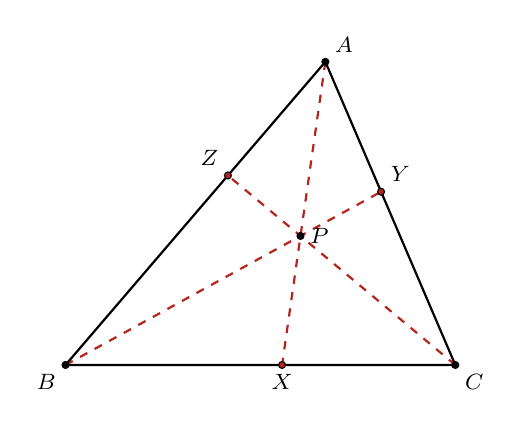
\begin{tikzpicture}[scale=0.55]
    \coordinate (A) at (6,7);
    \coordinate (B) at (0,0);
    \coordinate (C) at (9,0);
    \coordinate (X) at (5,0);
    \coordinate (Y) at (7.28565016637005,4.000149611803217);
    \coordinate (Z) at (3.7501227278585287,4.375143182501617);
    \coordinate (P) at (5.425553249578132,2.978872747046927);

    \draw[thick] (A) -- (B) -- (C) -- cycle;
    \draw[thick,dashed,BrickRed] (A) -- (X);
    \draw[thick,dashed,BrickRed] (B) -- (Y);
    \draw[thick,dashed,BrickRed] (C) -- (Z);

    \draw[fill=black] (A) circle (0.08)
        node[above right] {\footnotesize $A$};
    \draw[fill=black] (B) circle (0.08)
        node[below left] {\footnotesize $B$};
    \draw[fill=black] (C) circle (0.08)
        node[below right] {\footnotesize $C$};
    \draw[fill=BrickRed] (X) circle (0.08)
        node[below] {\footnotesize $X$};
    \draw[fill=BrickRed] (Y) circle (0.08)
        node[above right] {\footnotesize $Y$};
    \draw[fill=BrickRed] (Z) circle (0.08)
        node[above left] {\footnotesize $Z$};
    \draw[fill=black] (P) circle (0.08)
        node[right] {\footnotesize $P$};
\end{tikzpicture}
\end{figure}

Here, the lines $AX, BY, CZ$ are also known as cevians. Because this
is also a very popular theorem and I assume we are somewhat
familiar with this theorem, let's move on to a slightly less
popular form of this theorem.

Continuing with Ceva's standard form, there is also angle version.
This is very popular in Korea and we have a special name for it
as well, but for some reason, I don't think this is very well known
internationally. Some sources call this as Trigonometric Form of
Ceva's Theorem, but let's call it as Angle Form of Ceva's Theorem
because that's easier to pronounce.

\begin{corollary}
{Angle Form of Ceva's Theorem}
{Angle Form of Ceva's Theorem}
Given a triangle $ABC$, let $X, Y, Z$ be points on lines $BC, CA, AB$
respectively. The lines $AX, BY, CZ$ are concurrent at $P$ if and
only if the following equation holds.
\[
\frac{\sin(\angle{BAX})}{\sin(\angle{CAX})}
\cdot \frac{\sin(\angle{CBY})}{\sin(\angle{ABY})}
\cdot \frac{\sin(\angle{ACZ})}{\sin(\angle{BCZ})}
= 1
\]
\end{corollary}

This corollary powered with trigonometric identities can become
very powerful. Future notes includes some of its applications
in different topics like isogonal conjugate. Generally I think
we do need to show this corollary during exams, but I think it
is pretty self evident considering area of the triangles.
Next up we have Ptolemy's Theorem!

\begin{theorem}{Ptolemy's Theorem}{Ptolemy's Theorem}
Given a cyclic quadrilateral $ABCD$, the following equation holds.
\[
AC \cdot BD = AB \cdot DC + BC \cdot DA
\]
\end{theorem}

I personally have not seen many application of Ptolemy's Theorem
for KMO, but I think it appears quite often in KJMO. This is
pretty much it for the theorem and I think because most of us
are aware of this theorem, let's review our final theorem.

\begin{theorem}{Apollonius' Theorem}{Apollonius' Theorem}
Given a triangle $ABC$ with midpoint $M$ of $BC$, the following
equation holds.
\[
AB^2 + AC^2 = 2(BM^2 + AM^2)
\]
\end{theorem}

This has a special name, but it is just Stewart's theorem applied
to a midpoint $M$.

This is it for this section! Here I listed some of the foundational
topics that we must know before proceeding to latter notes,
and although there wasn't rigorous explanation with examples for
each theorem, I hope it was a good reminder of some of the topics!
As mentioned previously, olympiad geometry requires lots of background
knowledge to solve problems, and these are only the surface of them.
But before we move on to more exciting topics, let's review some of
the topics form Number Theory as well.

\end{document}


